\section{Diseño y construcción de la maqueta}

La estructura física fue diseñada para corte láser y posteriormente ensamblada en MDF mediante uniones de pestañas y ranuras. El diseño distribuye el recorrido del automóvil en una base alargada con paredes laterales, zonas superiores para sostener los elementos de proceso y una caja inferior destinada al mecanismo de transporte.

Los archivos de fabricación incluyen la base, paredes laterales, paneles con ventanas y perforaciones, soportes del depósito y piezas específicas para el montaje de sensores y actuadores. La geometría de corte incorpora las ranuras necesarias para el ensamble y aberturas para el paso de ejes, cables y elementos de sensado.

\begin{figure}[H]
    \centering
    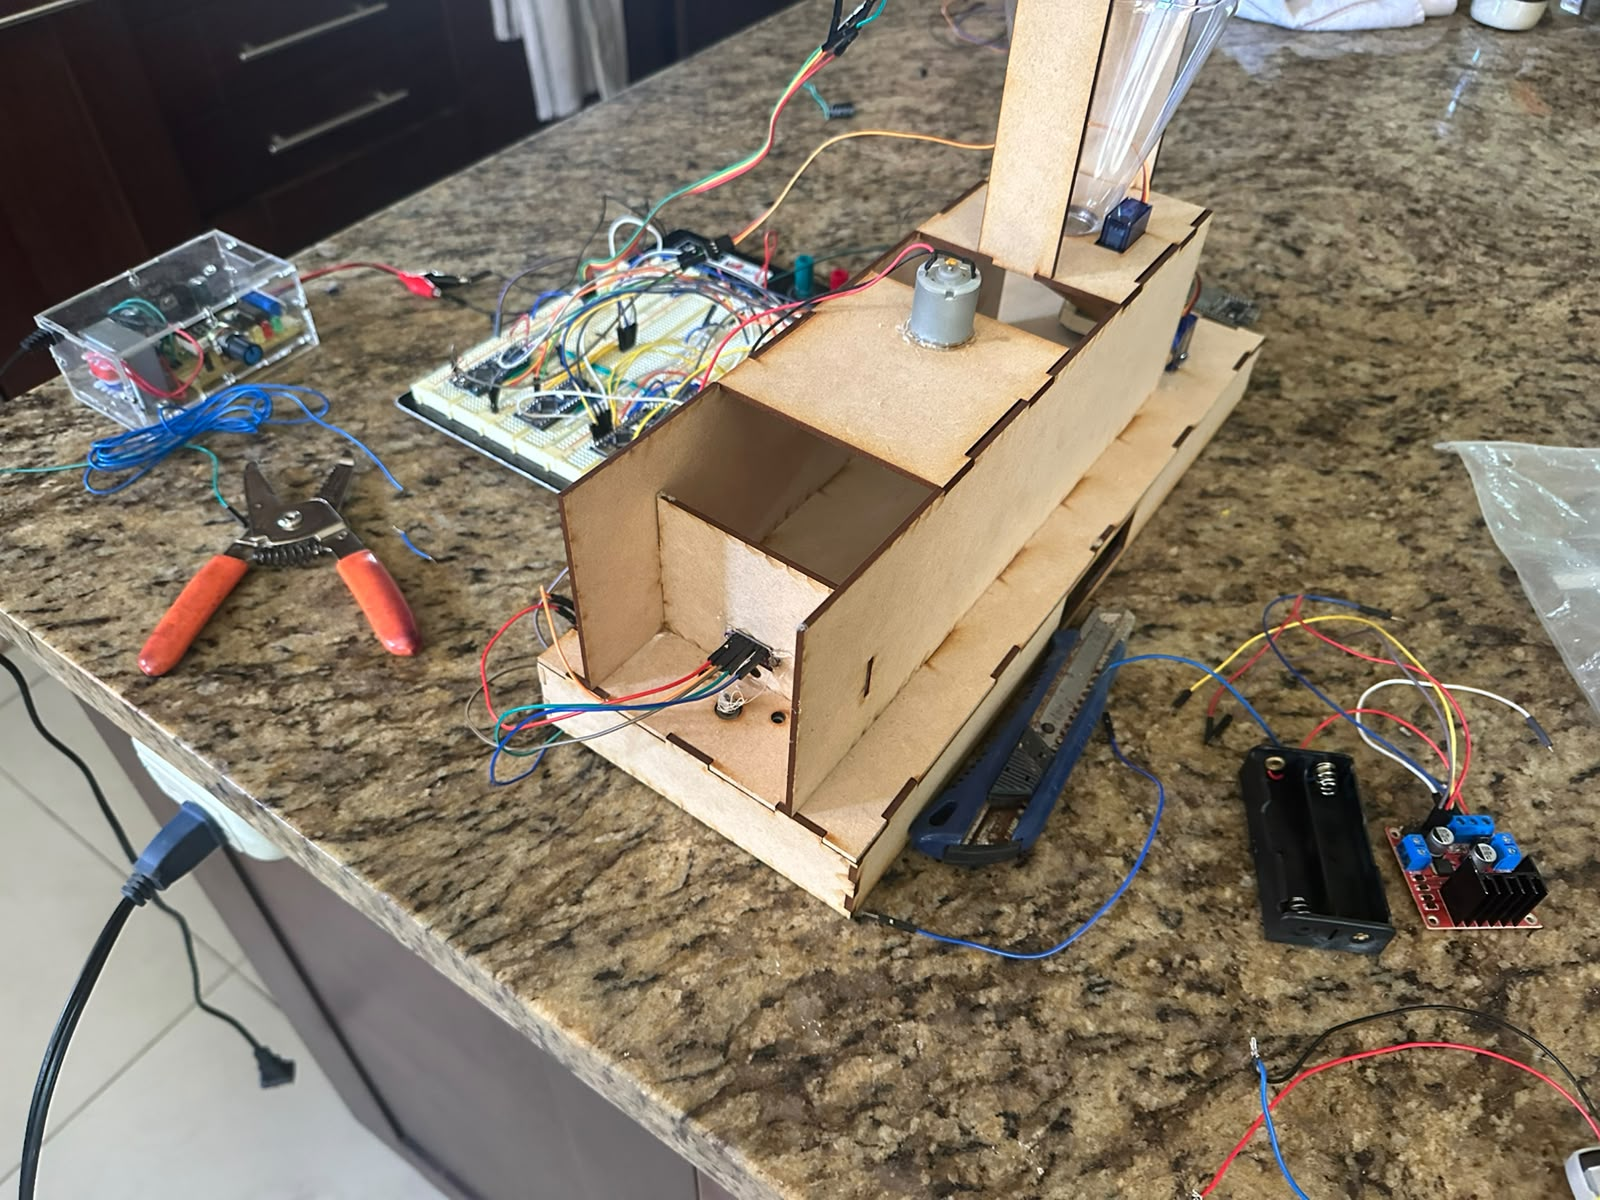
\includegraphics[width=0.88\textwidth]{imagenes/prototipo_perspectiva.jpeg}
    \caption{Vista general del prototipo físico del Car Wash ensamblado en MDF.}
\end{figure}

En el prototipo construido se observa el depósito elevado, la estructura vertical que lo sostiene, el motor DC instalado sobre una de las secciones superiores y el recorrido interior del vehículo. La electrónica de control se mantuvo externamente sobre protoboard, lo que facilita la depuración y modificación del cableado durante el desarrollo.

\begin{figure}[H]
    \centering
    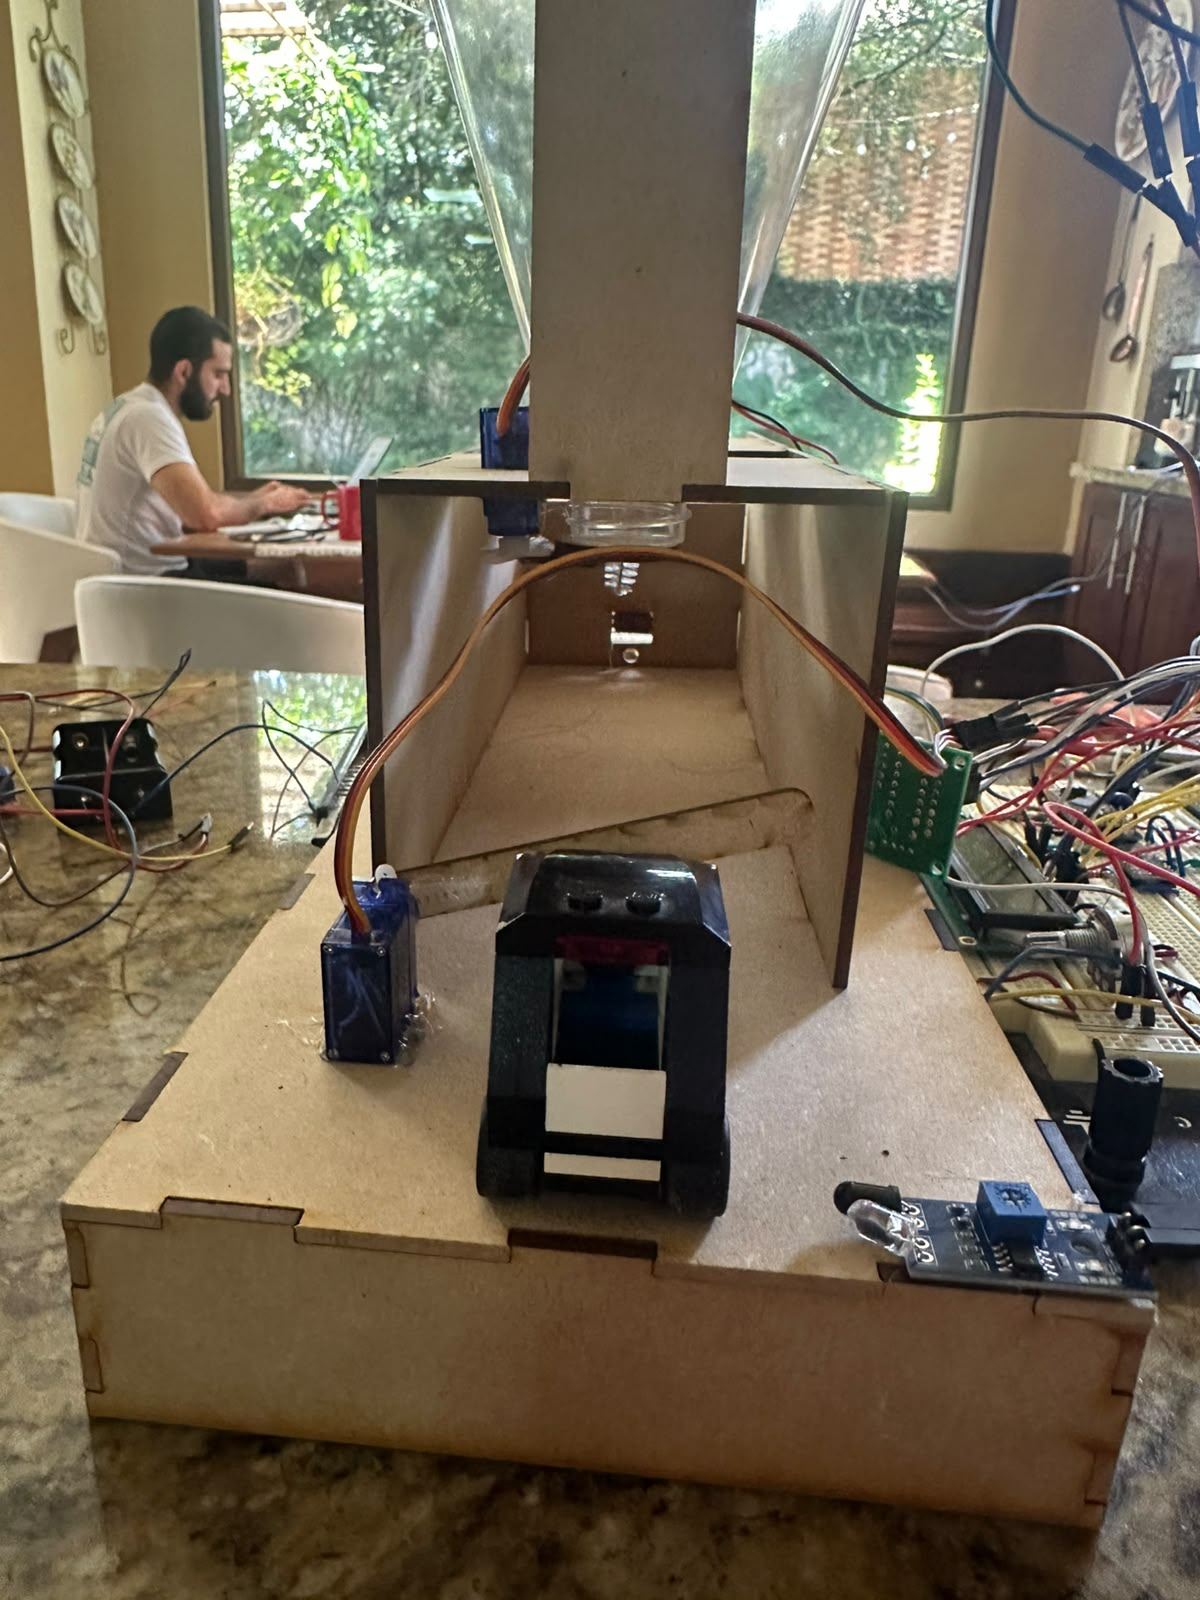
\includegraphics[width=0.82\textwidth]{imagenes/prototipo_entrada_frontal.jpeg}
    \caption{Entrada del Car Wash con vehículo, servomotor de puerta y sensor infrarrojo.}
\end{figure}

La entrada incorpora el vehículo de prueba, el servomotor que acciona la barrera y el módulo infrarrojo utilizado para detectar la presencia inicial. En la parte interior puede observarse el canal de recorrido y la abertura longitudinal asociada al mecanismo que desplaza el automóvil.

\begin{figure}[H]
    \centering
    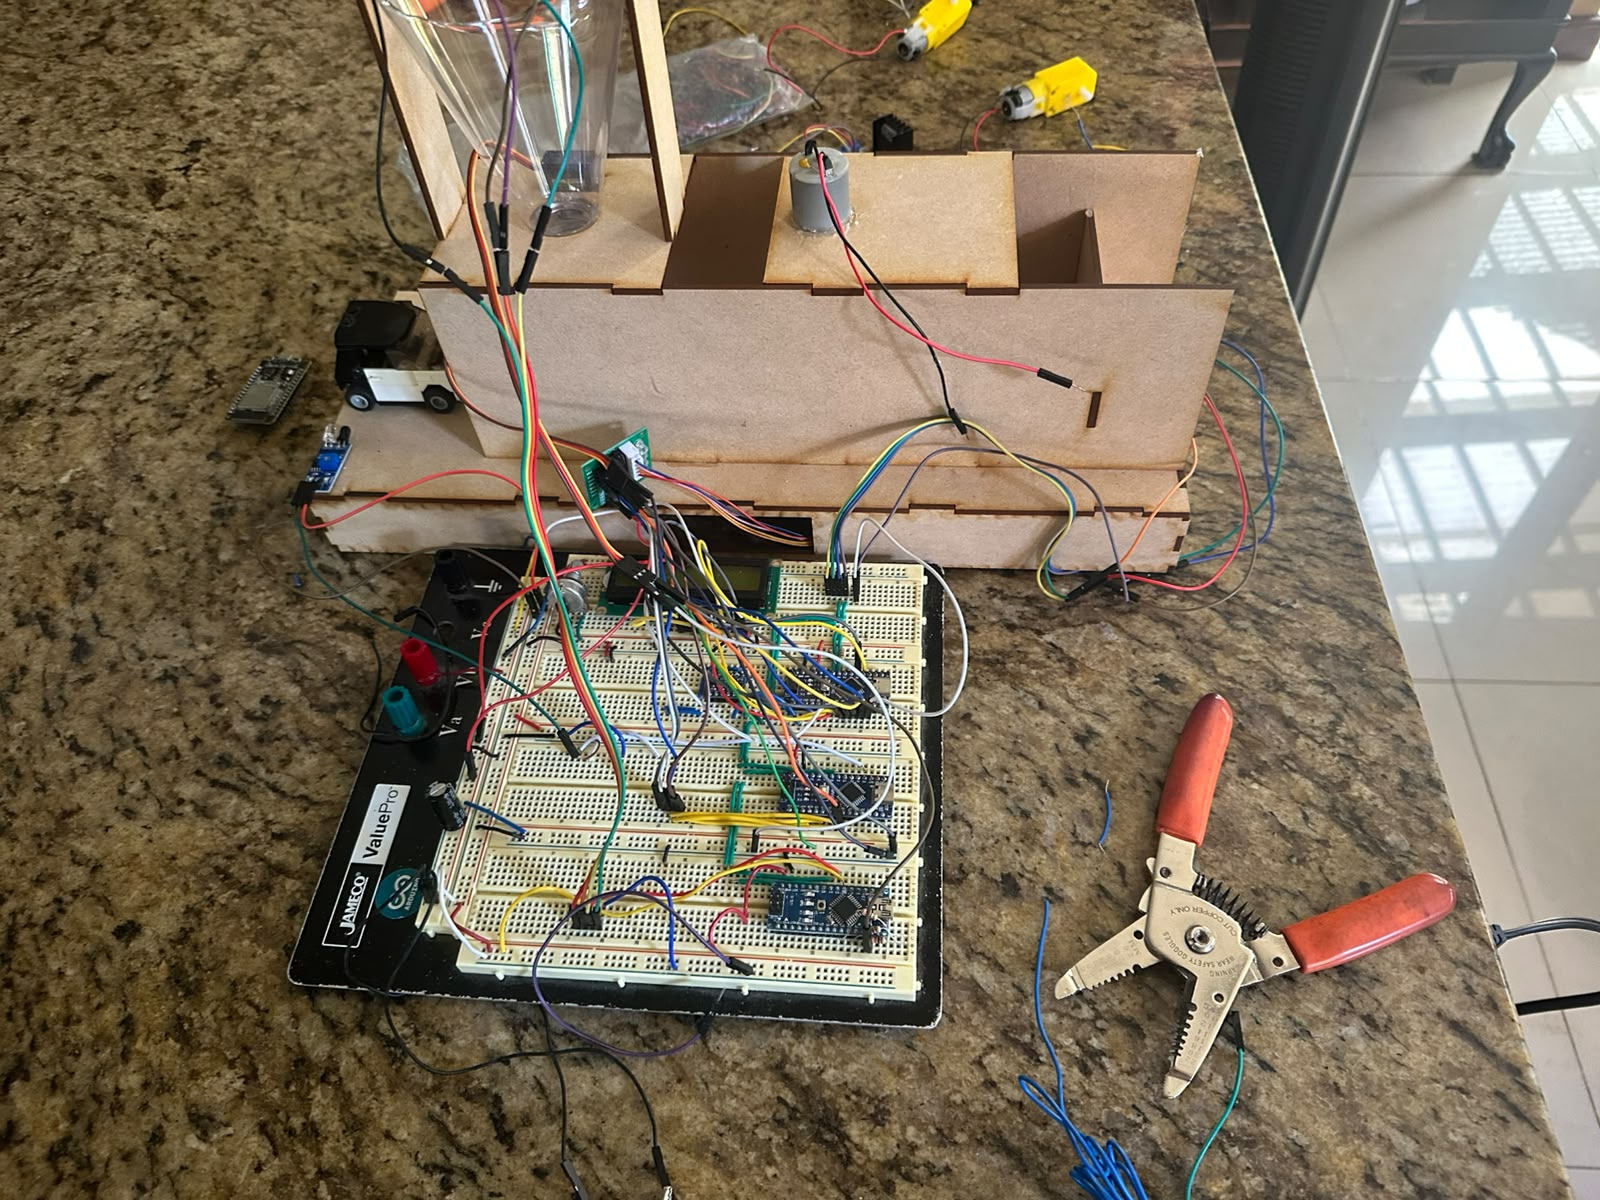
\includegraphics[width=0.88\textwidth]{imagenes/prototipo_electronica.jpeg}
    \caption{Prototipo conectado a la electrónica de control durante la etapa de integración.}
\end{figure}

Las fotografías corresponden a una etapa de integración y pruebas, por lo que el cableado mostrado no representa necesariamente el acabado final de presentación. Sin embargo, documentan la construcción real y la integración física de la maqueta con los microcontroladores y dispositivos.

\subsection{Integración electrónica final}
Durante la etapa final de integración, los tres Arduino Nano y el ESP32 fueron montados sobre la misma plataforma de prototipado junto con la pantalla LCD y el cableado de comunicación y alimentación. Esta disposición permitió verificar el sistema completo con los controladores conectados simultáneamente a la maqueta.

\begin{figure}[H]
    \centering
    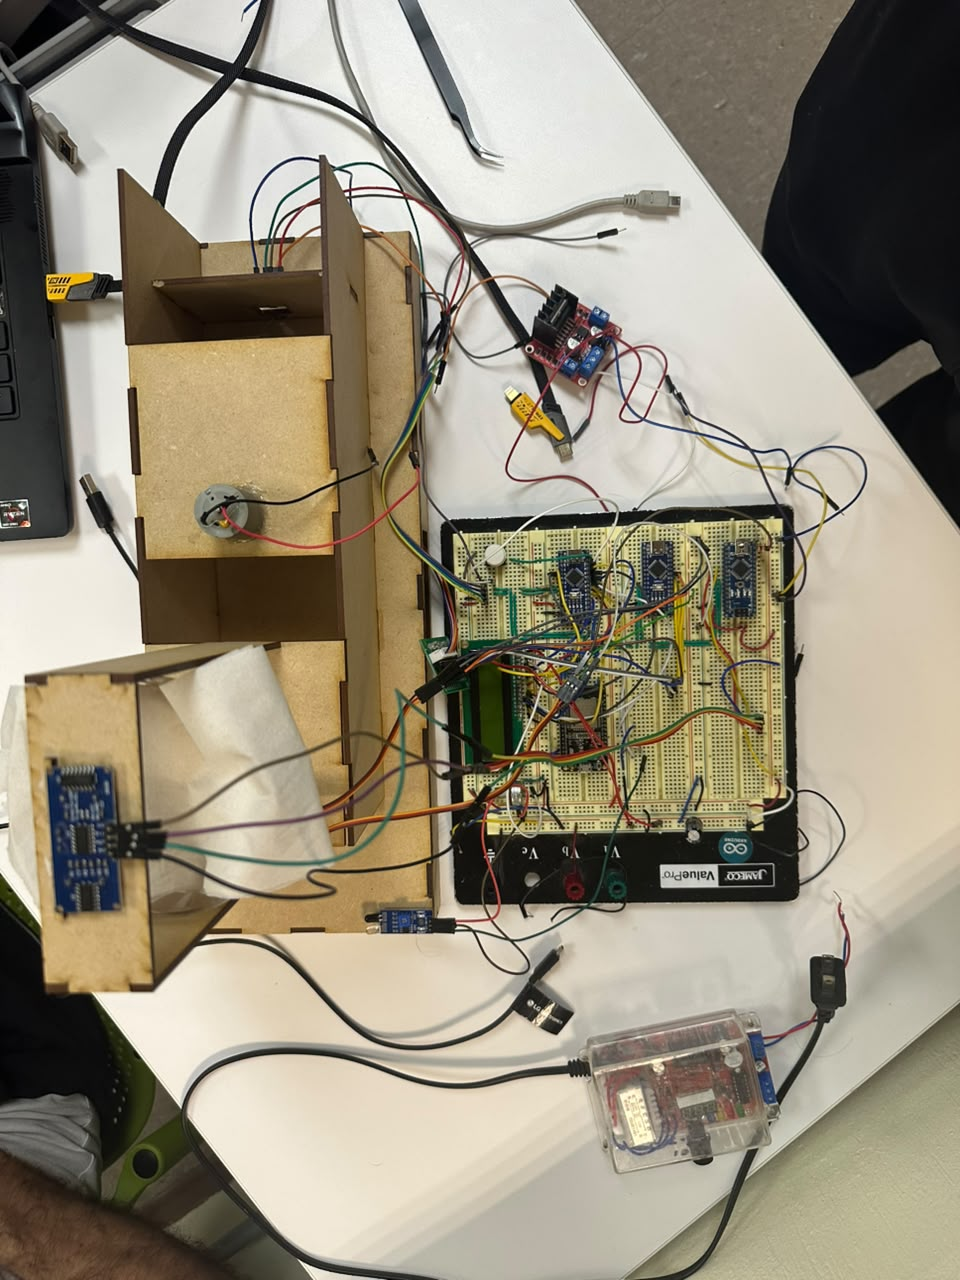
\includegraphics[width=0.82\textwidth]{imagenes/electronica_completa.jpeg}
    \caption{Vista superior de la maqueta y de la plataforma electrónica durante la integración final.}
\end{figure}

La siguiente fotografía permite observar con mayor detalle la distribución de los microcontroladores, el ESP32 y la pantalla LCD. El montaje se mantuvo en protoboard debido a que el proyecto se encontraba en etapa de pruebas e integración, facilitando modificaciones en las conexiones sin alterar la estructura mecánica.

\begin{figure}[H]
    \centering
    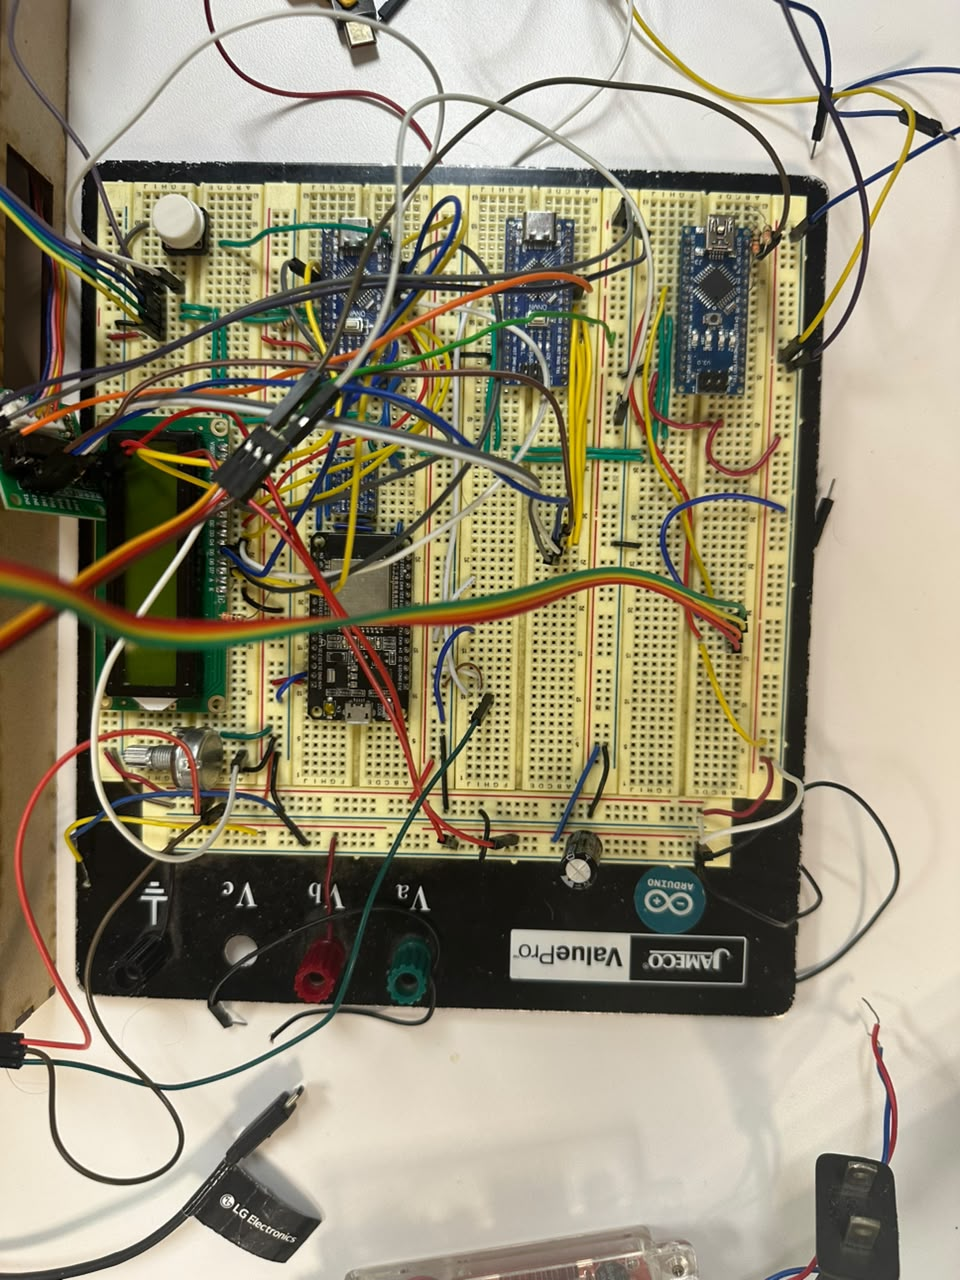
\includegraphics[width=0.72\textwidth]{imagenes/electronica_detalle.jpeg}
    \caption{Detalle de la plataforma de control con los ATmega328P, ESP32 y LCD utilizados en el prototipo.}
\end{figure}
